\documentclass[11pt,a4paper]{article}
\usepackage[margin=1in]{geometry}
\usepackage[T1]{fontenc}
\usepackage[utf8]{inputenc}
\usepackage{lmodern}
\usepackage{hyperref}
\usepackage{enumitem}
\usepackage{xurl}
\usepackage{tikz}
\usepackage{float}
\usetikzlibrary{arrows.meta, positioning, shapes.geometric}
\hypersetup{colorlinks=true,linkcolor=blue,urlcolor=blue}
\newcommand{\codepath}[1]{\path{#1}}
\tikzset{
  box/.style={rectangle,draw,rounded corners,align=center,inner sep=3pt,minimum width=44mm},
  decision/.style={diamond,draw,aspect=2.2,align=center,inner sep=2pt},
  line/.style={-Latex}
}

\title{Phase-2 Spike: Deliverable 7 (Parameter Sweep Runner)}
\author{SIT Engine Documentation}
\date{\today}

\begin{document}
\maketitle

\section{Technical Description}
This deliverable enables controlled sweep experiments for Spike while preserving clean separation between experiment metadata and core SIT schema outputs.

\section{Implementation Fulfillment}
Implemented in \codepath{Phase-2/sweeps/run_param_sweep.py} via \texttt{load\_config()}, \texttt{build\_cases()}, \texttt{to\_cmd()}, \texttt{run\_case()}, and \texttt{main()}. 

\section{Design \& Architecture}
\subsection*{Function Attributes}
\begin{itemize}[leftmargin=*]
  \item \texttt{load\_config()}: Inputs=config path; Outputs=shared+matrix config; Side effects=parses sweep definition; Failure modes=invalid JSON/schema.
  \item \texttt{build\_cases()}: Inputs=matrix parameters; Outputs=expanded case list; Side effects=constructs cartesian matrix; Failure modes=empty matrix.
  \item \texttt{to\_cmd()}: Inputs=case + shared options; Outputs=command argv; Side effects=maps case to runnable CLI; Failure modes=bad arg mapping.
  \item \texttt{run\_case()}: Inputs=command argv + cwd; Outputs=subprocess result; Side effects=executes one sweep case; Failure modes=non-zero rc.
  \item \texttt{main()}: Inputs=CLI options; Outputs=sweep CSV/JSON/log outputs; Side effects=orchestrates full sweep lifecycle; Failure modes=partial/failed runs.
\end{itemize}
\subsection*{Function Execution Details}
\begin{enumerate}[leftmargin=*]
  \item \texttt{load\_config()}
  \begin{itemize}[leftmargin=*]
    \item Input attributes: config path.
    \item Processing flow: parses sweep definition.
    \item Output attributes: shared+matrix config.
    \item Failure behavior: invalid JSON/schema.
  \end{itemize}
  \item \texttt{build\_cases()}
  \begin{itemize}[leftmargin=*]
    \item Input attributes: matrix parameters.
    \item Processing flow: constructs cartesian matrix.
    \item Output attributes: expanded case list.
    \item Failure behavior: empty matrix.
  \end{itemize}
  \item \texttt{to\_cmd()}
  \begin{itemize}[leftmargin=*]
    \item Input attributes: case + shared options.
    \item Processing flow: maps case to runnable CLI.
    \item Output attributes: command argv.
    \item Failure behavior: bad arg mapping.
  \end{itemize}
  \item \texttt{run\_case()}
  \begin{itemize}[leftmargin=*]
    \item Input attributes: command argv + cwd.
    \item Processing flow: executes one sweep case.
    \item Output attributes: subprocess result.
    \item Failure behavior: non-zero rc.
  \end{itemize}
  \item \texttt{main()}
  \begin{itemize}[leftmargin=*]
    \item Input attributes: CLI options.
    \item Processing flow: orchestrates full sweep lifecycle.
    \item Output attributes: sweep CSV/JSON/log outputs.
    \item Failure behavior: partial/failed runs.
  \end{itemize}
\end{enumerate}


\subsection*{Diagram A: End-to-End Design Flow}
\begin{figure}[H]
\centering
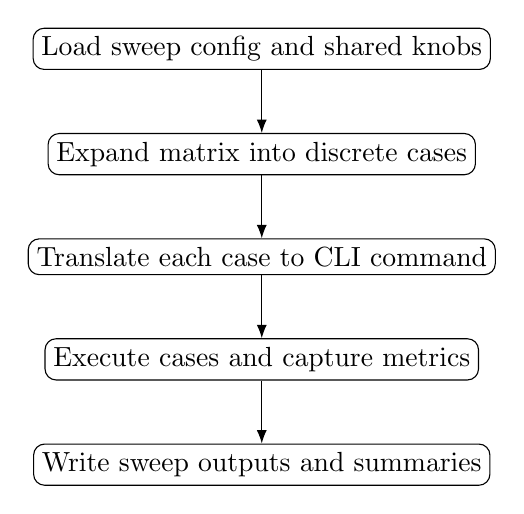
\begin{tikzpicture}[node distance=8mm and 12mm]
\node[box] (a) {Load sweep config and shared knobs};
\node[box, below=of a] (b) {Expand matrix into discrete cases};
\node[box, below=of b] (c) {Translate each case to CLI command};
\node[box, below=of c] (d) {Execute cases and capture metrics};
\node[box, below=of d] (e) {Write sweep outputs and summaries};
\draw[line] (a) -- (b);
\draw[line] (b) -- (c);
\draw[line] (c) -- (d);
\draw[line] (d) -- (e);
\end{tikzpicture}
\caption{Spike Deliverable 07: End-to-End Design Flow}
\end{figure}

\subsection*{Diagram B: Function Interaction and Attribute Flow}
\begin{figure}[H]
\centering
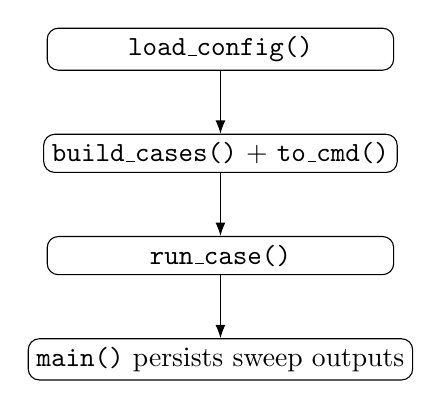
\begin{tikzpicture}[node distance=8mm and 12mm]
\node[box] (fa) {\texttt{load\_config()}};
\node[box, below=of fa] (fb) {\texttt{build\_cases()} + \texttt{to\_cmd()}};
\node[box, below=of fb] (fc) {\texttt{run\_case()}};
\node[box, below=of fc] (fd) {\texttt{main()} persists sweep outputs};
\draw[line] (fa) -- (fb);
\draw[line] (fb) -- (fc);
\draw[line] (fc) -- (fd);
\end{tikzpicture}
\caption{Spike Deliverable 07: Function Interaction and Attribute Flow}
\end{figure}

\end{document}
